\documentclass[twoside]{book}

% Packages required by doxygen
\usepackage{fixltx2e}
\usepackage{calc}
\usepackage{doxygen}
\usepackage[export]{adjustbox} % also loads graphicx
\usepackage{graphicx}
\usepackage[utf8]{inputenc}
\usepackage{makeidx}
\usepackage{multicol}
\usepackage{multirow}
\PassOptionsToPackage{warn}{textcomp}
\usepackage{textcomp}
\usepackage[nointegrals]{wasysym}
\usepackage[table]{xcolor}

% Font selection
\usepackage[T1]{fontenc}
\usepackage[scaled=.90]{helvet}
\usepackage{courier}
\usepackage{amssymb}
\usepackage{sectsty}
\renewcommand{\familydefault}{\sfdefault}
\allsectionsfont{%
  \fontseries{bc}\selectfont%
  \color{darkgray}%
}
\renewcommand{\DoxyLabelFont}{%
  \fontseries{bc}\selectfont%
  \color{darkgray}%
}
\newcommand{\+}{\discretionary{\mbox{\scriptsize$\hookleftarrow$}}{}{}}

% Page & text layout
\usepackage{geometry}
\geometry{%
  a4paper,%
  top=2.5cm,%
  bottom=2.5cm,%
  left=2.5cm,%
  right=2.5cm%
}
\tolerance=750
\hfuzz=15pt
\hbadness=750
\setlength{\emergencystretch}{15pt}
\setlength{\parindent}{0cm}
\setlength{\parskip}{3ex plus 2ex minus 2ex}
\makeatletter
\renewcommand{\paragraph}{%
  \@startsection{paragraph}{4}{0ex}{-1.0ex}{1.0ex}{%
    \normalfont\normalsize\bfseries\SS@parafont%
  }%
}
\renewcommand{\subparagraph}{%
  \@startsection{subparagraph}{5}{0ex}{-1.0ex}{1.0ex}{%
    \normalfont\normalsize\bfseries\SS@subparafont%
  }%
}
\makeatother

% Headers & footers
\usepackage{fancyhdr}
\pagestyle{fancyplain}
\fancyhead[LE]{\fancyplain{}{\bfseries\thepage}}
\fancyhead[CE]{\fancyplain{}{}}
\fancyhead[RE]{\fancyplain{}{\bfseries\leftmark}}
\fancyhead[LO]{\fancyplain{}{\bfseries\rightmark}}
\fancyhead[CO]{\fancyplain{}{}}
\fancyhead[RO]{\fancyplain{}{\bfseries\thepage}}
\fancyfoot[LE]{\fancyplain{}{}}
\fancyfoot[CE]{\fancyplain{}{}}
\fancyfoot[RE]{\fancyplain{}{\bfseries\scriptsize Generated by Doxygen }}
\fancyfoot[LO]{\fancyplain{}{\bfseries\scriptsize Generated by Doxygen }}
\fancyfoot[CO]{\fancyplain{}{}}
\fancyfoot[RO]{\fancyplain{}{}}
\renewcommand{\footrulewidth}{0.4pt}
\renewcommand{\chaptermark}[1]{%
  \markboth{#1}{}%
}
\renewcommand{\sectionmark}[1]{%
  \markright{\thesection\ #1}%
}

% Indices & bibliography
\usepackage{natbib}
\usepackage[titles]{tocloft}
\setcounter{tocdepth}{3}
\setcounter{secnumdepth}{5}
\makeindex

% Hyperlinks (required, but should be loaded last)
\usepackage{ifpdf}
\ifpdf
  \usepackage[pdftex,pagebackref=true]{hyperref}
\else
  \usepackage[ps2pdf,pagebackref=true]{hyperref}
\fi
\hypersetup{%
  colorlinks=true,%
  linkcolor=blue,%
  citecolor=blue,%
  unicode%
}

% Custom commands
\newcommand{\clearemptydoublepage}{%
  \newpage{\pagestyle{empty}\cleardoublepage}%
}

\usepackage{caption}
\captionsetup{labelsep=space,justification=centering,font={bf},singlelinecheck=off,skip=4pt,position=top}

%===== C O N T E N T S =====

\begin{document}

% Titlepage & ToC
\hypersetup{pageanchor=false,
             bookmarksnumbered=true,
             pdfencoding=unicode
            }
\pagenumbering{alph}
\begin{titlepage}
\vspace*{7cm}
\begin{center}%
{\Large Blackjack \\[1ex]\large 2.\+0 }\\
\vspace*{1cm}
{\large Generated by Doxygen 1.8.14}\\
\end{center}
\end{titlepage}
\clearemptydoublepage
\pagenumbering{roman}
\tableofcontents
\clearemptydoublepage
\pagenumbering{arabic}
\hypersetup{pageanchor=true}

%--- Begin generated contents ---
\chapter{Hierarchical Index}
\section{Class Hierarchy}
This inheritance list is sorted roughly, but not completely, alphabetically\+:\begin{DoxyCompactList}
\item \contentsline{section}{Card}{\pageref{class_card}}{}
\begin{DoxyCompactList}
\item \contentsline{section}{Normal\+Card}{\pageref{class_normal_card}}{}
\item \contentsline{section}{Special\+Card}{\pageref{class_special_card}}{}
\end{DoxyCompactList}
\item \contentsline{section}{Deck}{\pageref{class_deck}}{}
\end{DoxyCompactList}

\chapter{Class Index}
\section{Class List}
Here are the classes, structs, unions and interfaces with brief descriptions\+:\begin{DoxyCompactList}
\item\contentsline{section}{\mbox{\hyperlink{struct_card}{Card}} }{\pageref{struct_card}}{}
\item\contentsline{section}{\mbox{\hyperlink{struct_deck}{Deck}} }{\pageref{struct_deck}}{}
\end{DoxyCompactList}

\chapter{Class Documentation}
\hypertarget{class_card}{}\section{Card Class Reference}
\label{class_card}\index{Card@{Card}}
Inheritance diagram for Card\+:\begin{figure}[H]
\begin{center}
\leavevmode
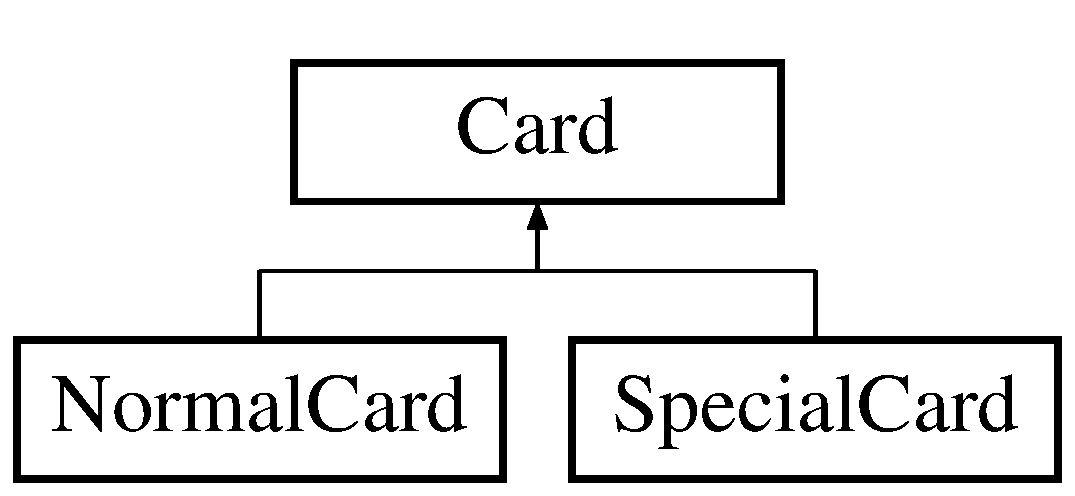
\includegraphics[height=2.000000cm]{class_card}
\end{center}
\end{figure}
\subsection*{Public Member Functions}
\begin{DoxyCompactItemize}
\item 
\mbox{\Hypertarget{class_card_a38da8da2b9f38a613f327a50cde3da34}\label{class_card_a38da8da2b9f38a613f327a50cde3da34}} 
string {\bfseries get\+Readable} ()
\item 
\mbox{\Hypertarget{class_card_ae6327dfb90c513f455c2e0db427cbcee}\label{class_card_ae6327dfb90c513f455c2e0db427cbcee}} 
virtual int {\bfseries get\+Value} ()
\item 
\mbox{\Hypertarget{class_card_a43f6f0bd60e577a7be3c58fa447f45e7}\label{class_card_a43f6f0bd60e577a7be3c58fa447f45e7}} 
int {\bfseries get\+Type} ()
\item 
\mbox{\Hypertarget{class_card_aa77888deaf592cad11eae8b28885d0d0}\label{class_card_aa77888deaf592cad11eae8b28885d0d0}} 
int {\bfseries operator+} (\mbox{\hyperlink{class_card}{Card}} \&)
\item 
\mbox{\Hypertarget{class_card_aef84e6680ad60e31734daf9e57deb69a}\label{class_card_aef84e6680ad60e31734daf9e57deb69a}} 
int {\bfseries operator-\/} (\mbox{\hyperlink{class_card}{Card}} \&)
\end{DoxyCompactItemize}
\subsection*{Protected Attributes}
\begin{DoxyCompactItemize}
\item 
\mbox{\Hypertarget{class_card_a68d1b935f3e4830af01fb9dba6c8220a}\label{class_card_a68d1b935f3e4830af01fb9dba6c8220a}} 
int {\bfseries suit}
\item 
\mbox{\Hypertarget{class_card_a57c4269cef032dac1f282c9b2be3be4d}\label{class_card_a57c4269cef032dac1f282c9b2be3be4d}} 
int {\bfseries value}
\item 
\mbox{\Hypertarget{class_card_ad7f5c3654b479f739fab1bcfed5e2765}\label{class_card_ad7f5c3654b479f739fab1bcfed5e2765}} 
int {\bfseries type}
\end{DoxyCompactItemize}


The documentation for this class was generated from the following files\+:\begin{DoxyCompactItemize}
\item 
C\+:/\+Users/\+Seth/\+Desktop/\+Project2/Card.\+h\item 
C\+:/\+Users/\+Seth/\+Desktop/\+Project2/Card.\+cpp\end{DoxyCompactItemize}

\hypertarget{class_deck}{}\section{Deck Class Reference}
\label{class_deck}\index{Deck@{Deck}}
\subsection*{Public Member Functions}
\begin{DoxyCompactItemize}
\item 
\mbox{\Hypertarget{class_deck_a5487610d44f13d27ef54c930e2bdadf9}\label{class_deck_a5487610d44f13d27ef54c930e2bdadf9}} 
{\bfseries Deck} (int)
\item 
\mbox{\Hypertarget{class_deck_ad85ed05a8321f9d1f0a2255dd1251473}\label{class_deck_ad85ed05a8321f9d1f0a2255dd1251473}} 
void {\bfseries deal} (\mbox{\hyperlink{class_deck}{Deck}} \&)
\item 
\mbox{\Hypertarget{class_deck_a02ae42f8f3aa795bffbb6e7f603be588}\label{class_deck_a02ae42f8f3aa795bffbb6e7f603be588}} 
void {\bfseries fill} ()
\item 
\mbox{\Hypertarget{class_deck_adc55458a86a0bc20b5006ddc4ff75f5e}\label{class_deck_adc55458a86a0bc20b5006ddc4ff75f5e}} 
void {\bfseries show} ()
\item 
\mbox{\Hypertarget{class_deck_ae5a1e52ab00ae5924f2bc6b730dba3eb}\label{class_deck_ae5a1e52ab00ae5924f2bc6b730dba3eb}} 
void {\bfseries shuffle} ()
\item 
\mbox{\Hypertarget{class_deck_ae7b88d69f0b9482389d9c6bf93124691}\label{class_deck_ae7b88d69f0b9482389d9c6bf93124691}} 
int {\bfseries best\+Sum} ()
\item 
\mbox{\Hypertarget{class_deck_aff55a8c6dc64c321b9198482e4a35d78}\label{class_deck_aff55a8c6dc64c321b9198482e4a35d78}} 
void {\bfseries show\+Sum} ()
\item 
\mbox{\Hypertarget{class_deck_a1361dd35348612d243dfc111432cd9e7}\label{class_deck_a1361dd35348612d243dfc111432cd9e7}} 
void {\bfseries add\+Card} (\mbox{\hyperlink{class_deck}{Deck}} \&)
\item 
\mbox{\Hypertarget{class_deck_a6551c710d28fba3b8f7a097c3c43a046}\label{class_deck_a6551c710d28fba3b8f7a097c3c43a046}} 
int {\bfseries operator+} (\mbox{\hyperlink{class_deck}{Deck}} \&)
\end{DoxyCompactItemize}
\subsection*{Public Attributes}
\begin{DoxyCompactItemize}
\item 
\mbox{\Hypertarget{class_deck_a8a6e5802d07c4e5181f624fbdd67f71f}\label{class_deck_a8a6e5802d07c4e5181f624fbdd67f71f}} 
int {\bfseries size}
\item 
\mbox{\Hypertarget{class_deck_aa5c2498afeda699034fd5feb50234092}\label{class_deck_aa5c2498afeda699034fd5feb50234092}} 
\mbox{\hyperlink{class_card}{Card}} $\ast$ {\bfseries cards}
\end{DoxyCompactItemize}
\subsection*{Static Public Attributes}
\begin{DoxyCompactItemize}
\item 
\mbox{\Hypertarget{class_deck_a364998d2d2bb52aa71df64dca9844254}\label{class_deck_a364998d2d2bb52aa71df64dca9844254}} 
static int {\bfseries num\+Cards} = 0
\end{DoxyCompactItemize}


The documentation for this class was generated from the following files\+:\begin{DoxyCompactItemize}
\item 
C\+:/\+Users/\+Seth/\+Desktop/\+Project2/Deck.\+h\item 
C\+:/\+Users/\+Seth/\+Desktop/\+Project2/Deck.\+cpp\end{DoxyCompactItemize}

\hypertarget{class_normal_card}{}\section{Normal\+Card Class Reference}
\label{class_normal_card}\index{Normal\+Card@{Normal\+Card}}
Inheritance diagram for Normal\+Card\+:\begin{figure}[H]
\begin{center}
\leavevmode
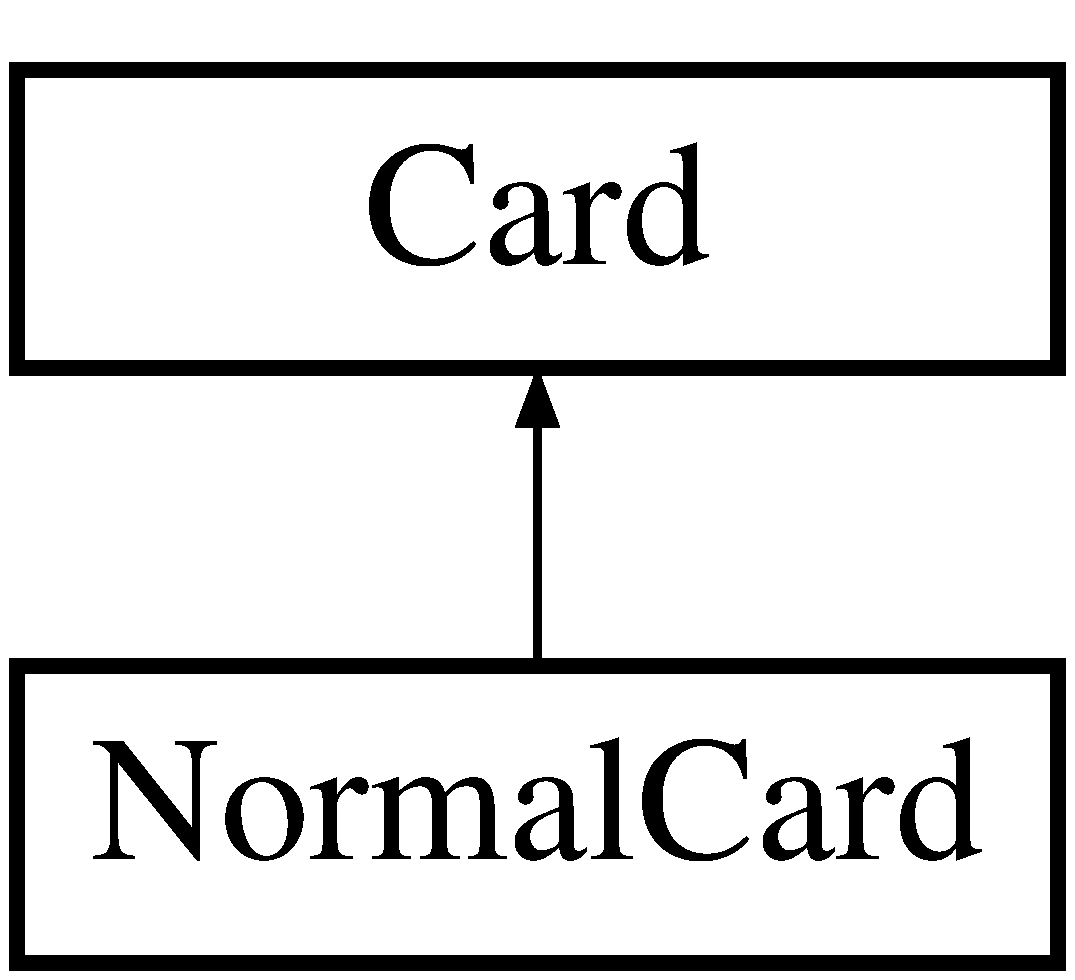
\includegraphics[height=2.000000cm]{class_normal_card}
\end{center}
\end{figure}
\subsection*{Public Member Functions}
\begin{DoxyCompactItemize}
\item 
\mbox{\Hypertarget{class_normal_card_afd7a293c0a5799f0bb4c336151e1f53e}\label{class_normal_card_afd7a293c0a5799f0bb4c336151e1f53e}} 
{\bfseries Normal\+Card} (int, int)
\end{DoxyCompactItemize}
\subsection*{Additional Inherited Members}


The documentation for this class was generated from the following files\+:\begin{DoxyCompactItemize}
\item 
C\+:/\+Users/\+Seth/\+Desktop/\+Project2/Normal\+Card.\+h\item 
C\+:/\+Users/\+Seth/\+Desktop/\+Project2/Normal\+Card.\+cpp\end{DoxyCompactItemize}

\hypertarget{class_special_card}{}\section{Special\+Card Class Reference}
\label{class_special_card}\index{Special\+Card@{Special\+Card}}
Inheritance diagram for Special\+Card\+:\begin{figure}[H]
\begin{center}
\leavevmode
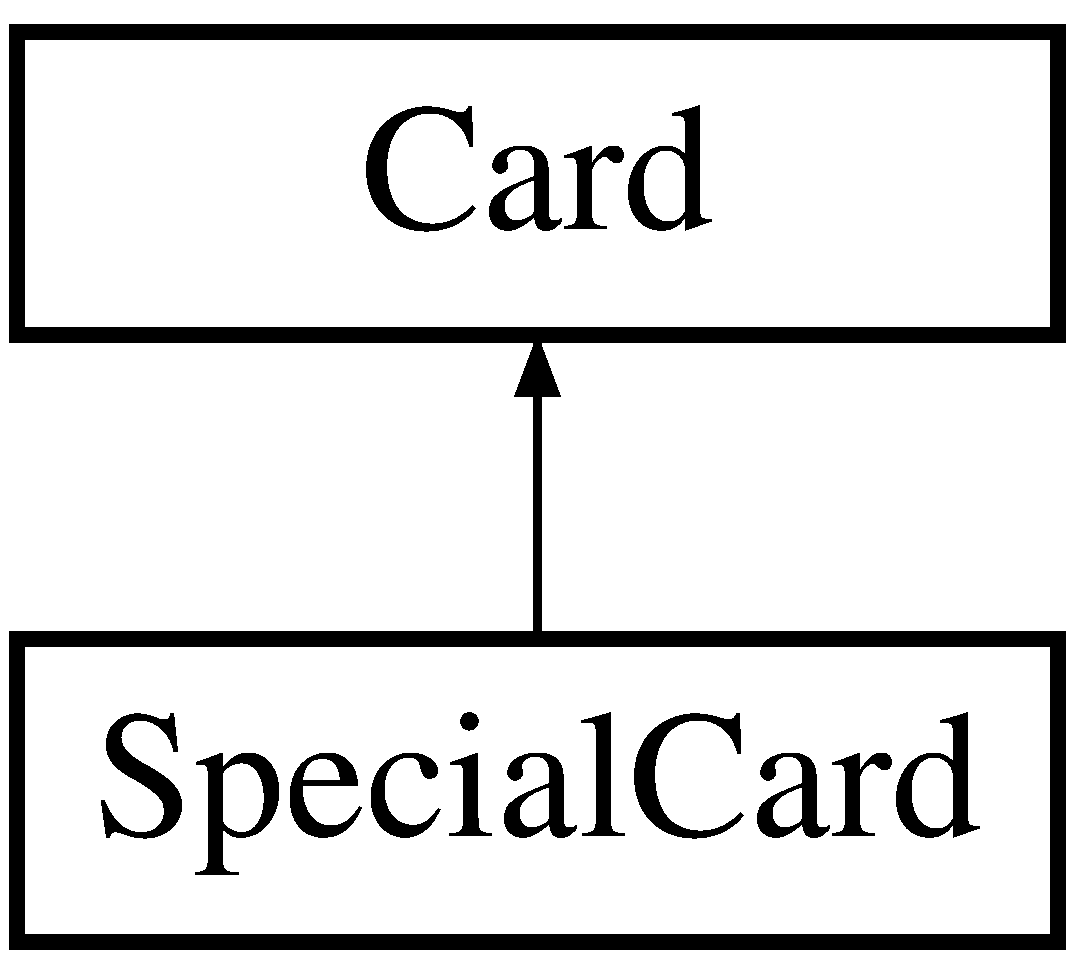
\includegraphics[height=2.000000cm]{class_special_card}
\end{center}
\end{figure}
\subsection*{Public Member Functions}
\begin{DoxyCompactItemize}
\item 
\mbox{\Hypertarget{class_special_card_a5f02d11446f822747fef386e53036dd8}\label{class_special_card_a5f02d11446f822747fef386e53036dd8}} 
{\bfseries Special\+Card} (int, int)
\item 
\mbox{\Hypertarget{class_special_card_ac29202fc09bf1c5b62c23869ce0a32ad}\label{class_special_card_ac29202fc09bf1c5b62c23869ce0a32ad}} 
int {\bfseries get\+Value} ()
\end{DoxyCompactItemize}
\subsection*{Additional Inherited Members}


The documentation for this class was generated from the following files\+:\begin{DoxyCompactItemize}
\item 
C\+:/\+Users/\+Seth/\+Desktop/\+Project2/Special\+Card.\+h\item 
C\+:/\+Users/\+Seth/\+Desktop/\+Project2/Special\+Card.\+cpp\end{DoxyCompactItemize}

%--- End generated contents ---

% Index
\backmatter
\newpage
\phantomsection
\clearemptydoublepage
\addcontentsline{toc}{chapter}{Index}
\printindex

\end{document}
